\chapter{Related Work}\label{ch:relatedwork}
\section{Large-scale Personal Fabrication}
Large-scale personal fabrication has been a topic in research for a long time. Especially in the metal industry and architecture, scaled-up machinery, such as concrete 3D printers, are used for additive manufacturing. The Denmark-based company \textit{3D Printhuset}\footnote{https://3dprinthuset.dk/} offers a product called \textit{building-on-demand}. Using a 6m x 6m x 3m concrete printer, the company printed a small office building within 50 hours.\\
\begin{figure}[h!]
    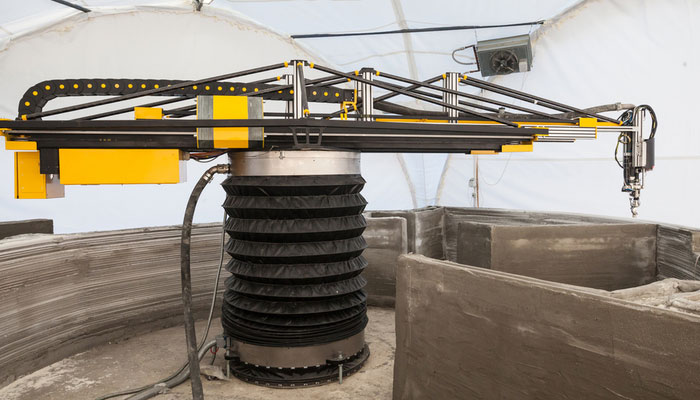
\includegraphics[width=.7\textwidth]{RelatedWork/concrete_3d_printer.jpg}
    \centering
    \caption{Apis Cor’s concrete 3D printer can create a house in 24 hours.}
    \label{fig:concrete_3d_printer}
\end{figure}
Instead of making the printer bigger, other solutions work by breaking up the object into smaller parts and print them on desktop machines.\\
3D printers use a fixed frame the print head moves on, limiting the size of the printed object to the size of the frame. To work around this limitation, researchers proposed techniques to place the print head on a mobile platform or make it fly by hanging it from a drone.\\
Yet another approach is to use human assisted devices, such as Protopiper.

\section{Construction Kits}
Construction kits are used for fast prototyping and fabrication. Prefabricated elements can be combined generically in various ways, depending on the desired outcome. The ZomeTool by Henrik and Kobbelt (TODO: Reference) is a mathematical modeling kit that can accurately approximate complex shapes, such as the Stanford Bunny. Skouras et al. (TODO: Reference) created an interactive editor to computationally combine interlocking elements into a desired shape.
\begin{figure}[h!]
    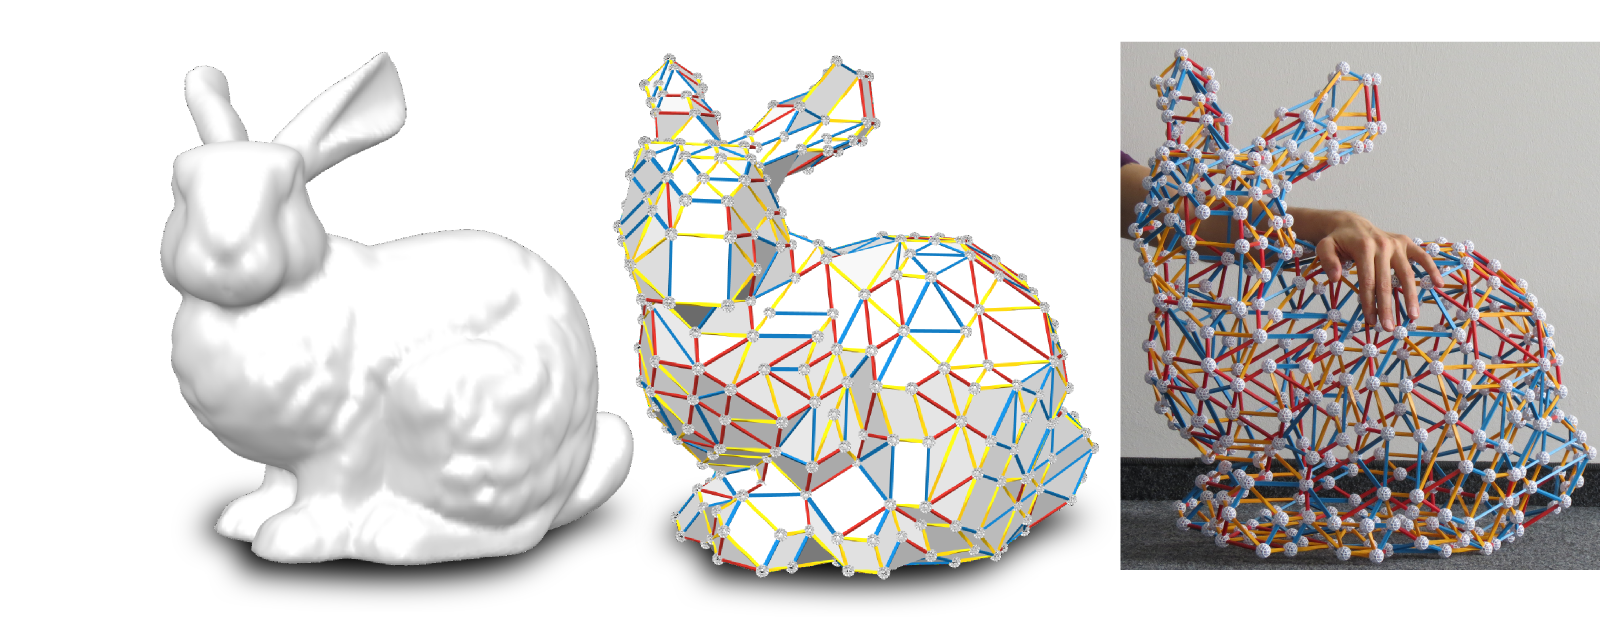
\includegraphics[width=.7\textwidth]{RelatedWork/bunnies.png}
    \centering
    \caption{The Stanford Bunny modeled with the ZomeTool construction kit.}
    \label{fig:bunnies}
\end{figure}

\section{Prototyping with Ready-Made Objects}
MixFab [33], and Encore [3] allow users to integrate existing objects into their design. For creating objects enclosing electronic components Ashbrook et al. [2] developed an augmented fabrication system. Devendorf and Ryokai [6] proposed a human-assisted fabrication system that helps users incorporate everyday objects into 3D print. Beady [10] approximates models from beads and offers an editor for refining them.\\
Gellért assembled wooden boards combined with 3D printed connectors in node-link structure [8]. Combining carbon tubes with 3D printed metal has been proposed for creating functional cars [40].
Skilled individuals have stacked or tied plastic bottles in order to make art pieces, furniture, rafts or houses [39]. Yamada et al. [36] proposed a system for arranging ready-made objects into 3D shapes using 3D-printed connectors.

\section{Building with Variable Geometry Trusses}
Fumihiro Inoue (TODO: Reference (book Robotics and Automation in Construction, chapter 16)) proposes the use of variable geometry trusses (VGTs) to introduce flexible movement into otherwise static structures. First used in space technology (TODO: reference to Natori \& Miura,
1994), variable geometry trusses are widely used today.\\
One use case is the Stewart platform. A Stewart platform consists of six actuators. A pair of two attach to a base plate, and cross over to attach to a top plate as a pair with their respective other neighbor actuator. This setup allows motion with 6 degrees of freedom (DoF), while keeping the stability of a truss. It is used in situations where high inertial forces can occur, such as motion platforms.\\
VGTs are also widely used in robotics. Tetrobot (TODO: Reference) is built by chaining the tetrahedron edges with linear actuators, which unite at a vertex in a spherical joint. The design and mechanics behind this type of spherical joints have been extensively analyzed [30, 32]. Tetrobot was designed to enable robots to reconfigure into different usages by reusing the same basic primitives. Researchers and engineers have explored variations of this VGT design in different contexts, for example: space applications (TODO: Reference), reconfigurable robotic manipulators (TODO: Reference), and shape morphing trusses (TODO: Reference).\\
Other researchers introduced design variations in this basic cell, allowing the resulting structure to afford new qualities. For instance, the Spiral Zipper (TODO: Reference) is an extendable edge, based on extending a cylinder that allows for extreme expansion ratios (e.g., 14:1). Similarly, Pneumatic Reel Actuator (TODO: Reference) is based on a mechanism that extrudes and retracts a plastic (tape-like) tubing, to act as an actuator. The mechanism is designed to be lightweight and low-cost (\$4 USD) while being limited in its robustness.\\
TrussFormer takes inspiration from VGTs and builds on the conceptual design of Tetrobot. To this work, TrussFormer contributes a spherical joint design that is automatically generated based on the designed truss geometry.

\section{Software Pipeline for Animatronics}
Algorithmic tools can help users create moving mechanisms. For example, kinematic synthesis of mechanisms [34], or generation of personalized walking toys from a library of predefined template mechanisms [2]. These can be embedded in design support systems, for example, generating moving toys from motion input [42], or synthetized planar kinematic mechanisms from sketch-based motion input [9].\\
Several software tools directly help the manual design of linkage-based mechanisms, such as LinkageDesigner [48] and Mechanism Perfboard [15]. These tools sometimes include physical simulation of simple mechanisms (e.g., hinges); examples include Crayon Physics [50] and freeCAD [49].\\
Researchers in the domain of personal fabrication have started to investigate the effects of dynamic forces in the resulting models, such as balancing rotating objects [22], interactively designing model airplanes [39], and approximating the elastic behavior of 3D printed materials [7].\\
TrussFormer extends these approaches by using physical simulation interactively in its editor. This combination is necessary to provide an editor that embodies the domain knowledge needed to produce large scale animated truss structures.
